%%%%%%%%%%%%%%%%%%%%%%%%%%%%%%%%%%%%%%%%%%%%%%%%%%%%%%%%%%%%%%%%%%%%%%
%     File: ExtendedAbstract_resul.tex                               %
%     Tex Master: ExtendedAbstract.tex                               %
%%%%%%%%%%%%%%%%%%%%%%%%%%%%%%%%%%%%%%%%%%%%%%%%%%%%%%%%%%%%%%%%%%%%%%

\section{Experiments}
\label{sec:experiments}

This section presents a comprehensive experimental evaluation of Aerial-D that spans model training, cross-dataset generalization, and targeted ablations. We begin by outlining the RSRefSeg backbone and training configuration, then report cross-dataset results on established aerial referring expression segmentation datasets. Beyond aggregate performance, we also include: (i) ablation of expression enhancement strategies; (ii) ablation of historic-filter training; and (iii) qualitative comparison across language models (o3, base Gemma3, and our distilled Gemma3-Aerial model), coupled with a cost analysis of these alternatives.

\subsection{Model Architecture}
\label{subsec:model_architecture}

Evaluating Aerial-D demands a model that preserves the link between natural-language instructions and precise masks while handling densely packed aerial targets. RSRefSeg meets these requirements and already demonstrated state-of-the-art results on RRSIS-D\cite{liu2024rotated}. We reimplemented the architecture in PyTorch and verified those RRSIS-D gains before extending the system to Aerial-D, which confirmed that the design transfers reliably to new datasets.

Our reimplementation of RSRefSeg\cite{chen2025rsrefseg} mirrors the original component pairing: SigLIP2\cite{siglip2} supplies the image–text encoder and SAM\cite{sam} provides the mask decoder. We fine-tune both modules with Low-Rank Adaptation (LoRA)\cite{lora} layers placed on the query and value projections of each vision encoder block and on the query, key, value, and output projections of the text encoder. Two checkpoints appear throughout the experiments. RSRefSeg-b keeps SAM-ViT-Base and LoRA rank $r\=16$ for a lighter configuration, whereas RSRefSeg-l upgrades to SAM-ViT-Large with rank $r\=32$ to maximize capacity while preserving the same training recipe.

\subsection{Experimental Setup}
\label{subsec:experimental_setup}

Training adheres to the RSRefSeg recipe so that differences arise from the data rather than from custom optimization. Batches contain four samples with gradient accumulation of two steps, yielding an effective batch size of eight. All experiments run on a single NVIDIA RTX~A6000 GPU. The combined model uses \texttt{SigLIP2-SO400M} for language–vision encoding at 384×384 resolution and \texttt{SAM-ViT-Large} at 1024×1024 for mask decoding, with LoRA rank \(r\=32\) steering the adaptation. We employ AdamW\cite{adamw} with learning rate $1\times10^{-4}$, weight decay 0.01, polynomial decay (power 0.9), mixed precision, and gradient clipping at 1.0 to mirror the original training dynamics. During data preparation we apply the three historic filters from Section~\ref{subsec:historic_filters} to 20\% of training images in each non-historic dataset, replacing the selected samples with one filtered copy chosen uniformly at random so the model encounters degradations throughout training.

In order to keep the cross-dataset mix balanced, Aerial-D contributes only the \emph{LLM Visual Variations} subset highlighted in Section~\ref{subsec:ablation_studies}. That ablation shows this subset carries the strongest signal while still covering every target; limiting Aerial-D to these expressions keeps the millions of available sentences from overwhelming the four public datasets, each of which supplies only tens of thousands of annotations. The combined run therefore spans Aerial-D (LLM Visual Variations), RRSIS-D\cite{liu2024rotated}, NWPU-Refer\cite{yang2024large}, RefSegRS\cite{yuan2023rrsis}, and Urban1960SatSeg\cite{hao2025urban1960satseg}. Validation follows the official splits, and Aerial-D relies on the 405K-expression "combined-all" split, which is further broken down into instance targets and semantic regions in Table~\ref{tab:aeriald_variants}. To probe robustness we also evaluate fully filtered validation sets for Aerial-D, RRSIS-D, NWPU-Refer, and RefSegRS by converting every image with one of the three historic filters. Scores for those variants appear in the "Hist." columns.

\subsection{Evaluation Results}
\label{subsec:evaluation_results}

Tables~\ref{tab:aeriald_variants} and \ref{tab:combined_training_results} report validation results for the combined model trained jointly on all datasets. Both tables focus on mean IoU and overall IoU for the original validation splits alongside their historic-filtered counterparts, highlighting aggregate overlap rather than thresholded pass rates.

Table~\ref{tab:aeriald_variants} isolates Aerial-D and reports validation performance by target type. Instance targets correspond to explicit objects or groups, while the "All Targets" column aggregates both instance- and semantic-level references across the full 405K validation expressions. These values serve as baseline checkpoints for future work that evaluates new architectures on Aerial-D.

Across the external datasets in Table~\ref{tab:combined_training_results}, the RSRefSeg-b and RSRefSeg-l checkpoints remain competitive with previously published results despite being trained within a single unified pipeline. That schedule blends five datasets, applies historic filters to more than 20\% of the training imagery, and supervises both instance- and semantic-level targets drawn from Aerial-D. Historic columns illustrate that the LoRA-tuned RSRefSeg-l retains accuracy under simulated degradations, closing the gap between clean and historic imagery without requiring dataset-specific adjustments. The same table also foregrounds how the larger checkpoint strengthens overall IoU on RefSegRS and NWPU-Refer while maintaining the strong RRSIS-D performance reported in prior work.

The combined evaluation therefore remains competitive with published references across every dataset while providing reproducible Aerial-D baselines. The modest gap between the original and historic evaluations confirms that injecting filtered imagery during training delivers robustness without eroding accuracy on contemporary photographs.

\begin{table*}[t]
\centering
\caption{Aerial-D supervision variants evaluated on the validation split (historic scores in \textcolor{blue}{blue}; ``--'' denotes metrics that are not yet available).}
\label{tab:aeriald_variants}
\resizebox{\textwidth}{!}{%
\begin{tabular}{@{}l|cc|cc@{}}
\toprule
\multirow{2}{*}{\textbf{Model}} & \multicolumn{2}{c|}{\textbf{Instance Targets}} & \multicolumn{2}{c}{\textbf{All Targets}} \\
\cmidrule(lr){2-3} \cmidrule(lr){4-5}
 & \textbf{mIoU} & \textbf{oIoU} & \textbf{mIoU} & \textbf{oIoU} \\
\midrule
\textbf{RSRefSeg-b (ours)} & 49.78\% / \textcolor{blue}{46.82\%} & 63.44\% / \textcolor{blue}{61.12\%} & 49.78\% / \textcolor{blue}{46.82\%} & 63.44\% / \textcolor{blue}{61.12\%} \\
\bottomrule
\end{tabular}%
}
\end{table*}

\begin{table*}[t]
\centering
\caption{Cross-dataset validation results for RSRefSeg variants (ours) and published baselines (historic scores in \textcolor{blue}{blue}; ``--'' indicates metrics not reported in the cited work).}
\label{tab:combined_training_results}
\resizebox{\textwidth}{!}{%
\begin{tabular}{@{}l|cc|cc|cc|cc@{}}
\toprule
\multirow{2}{*}{\textbf{Model}} & \multicolumn{2}{c|}{\textbf{RefSegRS}} & \multicolumn{2}{c|}{\textbf{RRSIS-D}} & \multicolumn{2}{c|}{\textbf{NWPU-Refer}} & \multicolumn{2}{c}{\textbf{Urban1960SatSeg}} \\
\cmidrule(lr){2-3} \cmidrule(lr){4-5} \cmidrule(lr){6-7} \cmidrule(lr){8-9}
 & \textbf{mIoU} & \textbf{oIoU} & \textbf{mIoU} & \textbf{oIoU} & \textbf{mIoU} & \textbf{oIoU} & \textbf{mIoU} & \textbf{oIoU} \\
\midrule
\textbf{RSRefSeg-b (ours)} & 24.81\% / \textcolor{blue}{17.54\%} & 40.89\% / \textcolor{blue}{29.41\%} & 64.37\% / \textcolor{blue}{61.16\%} & 76.83\% / \textcolor{blue}{75.44\%} & 39.42\% / \textcolor{blue}{33.15\%} & 59.52\% / \textcolor{blue}{\textbf{56.56\%}} & \textbf{70.65\%} & \textbf{88.86\%} \\
\textbf{RSRefSeg-l (ours)} & 44.52\% / \textcolor{blue}{\textbf{36.03\%}} & 55.74\% / \textcolor{blue}{\textbf{45.74\%}} & \textbf{65.37\%} / \textcolor{blue}{\textbf{62.61\%}} & 76.33\% / \textcolor{blue}{\textbf{76.03\%}} & \textbf{45.75\%} / \textcolor{blue}{\textbf{39.11\%}} & 62.75\% / \textcolor{blue}{55.29\%} & 69.74\% & 88.73\% \\
\midrule
RMSIN\cite{liu2024rotated,yang2024large,chen2025rsrefseg} & \textbf{59.96\%} & \textbf{76.81\%} & 62.27\% & 76.50\% & 41.75\% & 62.66\% & -- & -- \\
RSRefSeg-b\cite{chen2025rsrefseg} & -- & -- & 63.68\% & 76.05\% & -- & -- & -- & -- \\
RSRefSeg-l\cite{chen2025rsrefseg} & -- & -- & 64.67\% & \textbf{77.24\%} & -- & -- & -- & -- \\
MRSNet\cite{yang2024large} & -- & -- & -- & -- & 44.86\% & \textbf{63.59\%} & -- & -- \\
Urban1960SatUSM\cite{hao2025urban1960satseg} & -- & -- & -- & -- & -- & -- & 68.80\% & -- \\
\bottomrule
\end{tabular}%
}
\end{table*}

\subsection{LLM Expression Generation Ablation}
\label{subsec:ablation_studies}

To measure how synthetic language affects segmentation, we retrain RSRefSeg on Aerial-D while isolating the different expression sources. The goal is to contrast the original rule-generated sentences against those produced by the LLM pipeline and determine which variants provide the strongest supervision. We adopt the lighter RSRefSeg-b configuration—SAM-ViT-Base with LoRA rank \(r\=16\)—so each run completes quickly while preserving the optimization settings from Section~\ref{subsec:experimental_setup}.

Using this setup, we train four separate models, each exposed to a distinct slice of Aerial-D: (i) \emph{Rule-based Only} retains the deterministic descriptions produced by the rule system; (ii) \emph{LLM Language Variations} relies on rewrites that diversify the wording while preserving the target; (iii) \emph{LLM Visual Variations} selects LLM augmentations that inject alternative visual cues; and (iv) \emph{Combined All} unites the three sources. Figure~\ref{fig:llm_enhancement_example} illustrates how the enhanced variants expand the phrasing beyond the rule-based baseline. We evaluate the resulting checkpoints on four validation sets without additional tuning: Aerial-D (using the 405K-expression validation split) and three external datasets—RefSegRS, RRSIS-D, and NWPU-Refer—to observe how each expression type supports generalization beyond the training distribution.

Table~\ref{tab:ablation_expression_types} summarizes the results and explicitly reports both the number of \emph{Samples} and \emph{Epochs} used per configuration. Looking across datasets, several consistent patterns emerge. On Aerial-D, the \emph{Combined All} configuration achieves the best accuracy, which is expected given that the validation distribution matches that training mixture. For the three external datasets, different subsets yield the strongest generalization: on RRSIS-D, the \emph{LLM Language Variations} run delivers the highest scores; on NWPU-Refer, emphasizing varied visual cues through \emph{LLM Visual Variations} is most beneficial; and on RefSegRS, uniting the three sources provides the best results. These outcomes highlight the breadth of ways to phrase referring expressions and show that leveraging LLMs to introduce targeted variety improves cross-dataset generalization.

In order to keep early stopping responsive to each subset, we monitor validation loss across the four runs and halt training as soon as it begins to rebound. Because the \emph{Combined All} subset is roughly three times larger than the others, its validation loss ticks upward immediately after the second epoch, so we stop that run at two epochs. The three smaller subsets continue improving through the fourth epoch before showing the same rise, allowing four full passes over their data. This schedule means that the language-variation and visual-variation models actually process fewer total samples than the combined run, yet they surpass it on RRSIS-D and NWPU-Refer. The outcome reveals that curated expression subsets can be more sample efficient than the full mixture, which is why the combined model in Section~\ref{subsec:evaluation_results} draws on the LLM Visual Variations split of Aerial-D. Beyond sample efficiency, constraining Aerial-D to that subset keeps the cross-dataset mix from being dominated by a single corpus whose expression pool would otherwise reach into the millions.

% Ablation expression types table with explicit epochs and samples
\begin{table*}[t]
\centering
\caption{Expression Enhancement Ablation Across Four Datasets}
\label{tab:ablation_expression_types}
\resizebox{\textwidth}{!}{%
\begin{tabular}{@{}lcc|cc|cc|cc|cc@{}}
\toprule
\multirow{2}{*}{\textbf{Training Configuration}} & \multirow{2}{*}{\textbf{Samples}} & \multirow{2}{*}{\textbf{Epochs}} & \multicolumn{2}{c|}{\textbf{Aerial-D}} & \multicolumn{2}{c|}{\textbf{RefSegRS}} & \multicolumn{2}{c|}{\textbf{RRSIS-D}} & \multicolumn{2}{c}{\textbf{NWPU-Refer}} \\
\cmidrule(lr){4-5} \cmidrule(lr){6-7} \cmidrule(lr){8-9} \cmidrule(lr){10-11}
 & & & % \textbf{Pass@0.7} & 
\textbf{mIoU} & \textbf{oIoU} & % \textbf{Pass@0.7} & 
\textbf{mIoU} & \textbf{oIoU} & % \textbf{Pass@0.7} & 
\textbf{mIoU} & \textbf{oIoU} & % \textbf{Pass@0.7} & 
\textbf{mIoU} & \textbf{oIoU} \\
\midrule
Rule-based Only & 371K & 4 & % 26.81\% & 
34.57\% & 39.31\% & % 2.55\% & 
3.73\% & 0.55\% & % 29.89\% & 
34.22\% & 36.46\% & % 13.62\% & 
16.78\% & 13.70\% \\
LLM Language Variations & 364K & 4 & % 36.39\% & 
46.45\% & 56.99\% & % \textbf{3.02\%} & 
5.75\% & 4.99\% & % \textbf{35.63\%} & 
\textbf{41.63\%} & \textbf{42.48\%} & % \textbf{16.90\%} & 
21.89\% & 16.68\% \\
LLM Visual Variations & 382K & 4 & % 35.75\% & 
46.54\% & 63.02\% & % 2.55\% & 
18.32\% & 8.37\% & % 20.86\% & 
31.78\% & 33.73\% & % 15.91\% & 
\textbf{24.68\%} & \textbf{29.22\%} \\
Combined All & 1,118K & 2 & % \textbf{39.54\%} & 
\textbf{49.33\%} & \textbf{64.30\%} & % 1.86\% & 
\textbf{18.80\%} & \textbf{8.58\%} & % 23.39\% & 
34.07\% & 34.80\% & % 15.91\% & 
24.57\% & 28.27\% \\
\bottomrule
\end{tabular}%
}
\end{table*}

\subsection{Distillation Ablation: Gemma3 vs. o3 Model Comparison}
\label{subsec:distillation_ablation}

This ablation measures how the generator choice inside the LLM enhancement stage affects expression quality and overall cost. We evaluate three options for producing the enhanced expressions: OpenAI’s o3, the off‑the‑shelf Gemma3‑12B, and the distilled Gemma3-Aerial model described in Section~\ref{subsec:llm_expression_generation} (see Figure~\ref{fig:llm_distillation}).

All three models are prompted and decoded in the same way so that differences stem from the generator rather than the interface. The base Gemma3 baseline frequently ignores the dual-task schema, hallucinates objects that are not present, and references the guiding bounding boxes inside the expression, which undermines segmentation training. Distillation sharply reduces those errors, producing grounded descriptions that resemble the o3 outputs while remaining accessible on local hardware.

Table~\ref{tab:cost_comparison} quantifies the practical impact. Running o3 across \(\sim\)300{,}000 targets would cost roughly \$6.2K, whereas the distilled Gemma3 produces comparable guidance for about \$26—roughly 238× cheaper because inference runs locally instead of via a commercial API. Figure~\ref{fig:distillation_comparison} illustrates why the student is worth training: the base Gemma3 hallucinates a second baseball diamond that does not exist, while the distilled variant stays aligned with the image and mirrors the grounded detail that o3 provides.

% Cost comparison table
\begin{table}[t]
\centering
\caption{Cost Analysis: Gemma3 vs. o3 Model for Large-Scale Annotation\protect\footnotemark}
\label{tab:cost_comparison}
\resizebox{\columnwidth}{!}{%
\begin{tabular}{@{}lcc@{}}
\toprule
\textbf{Model} & \textbf{Cost per request} & \textbf{Cost for 300K requests} \\
\midrule
o3 Model & \$0.020728 & \$6,218.32 \\
Distilled Gemma3 & \$0.000087 & \$26.01 \\
\midrule
\textbf{Savings} & \textbf{238× cheaper} & \textbf{\$6,192.31 (99.6\%)} \\
\bottomrule
\end{tabular}%
}
\end{table}
\footnotetext{Cost calculations based on API pricing — o3: \$2.00 per million input tokens, \$8.00 per million output tokens (OpenAI API platform); Gemma3-12B: \$0.035 per million input tokens, \$0.141 per million output tokens (OpenRouter inference provider). Average tokens per request: o3 (1,670.8 input, 2,173.3 output), Gemma3 (1,330.0 input, 284.7 output). Calculations based on 15 sample requests.}

\begin{figure*}[t]
\centering
\begin{minipage}{0.5\textwidth}
\centering
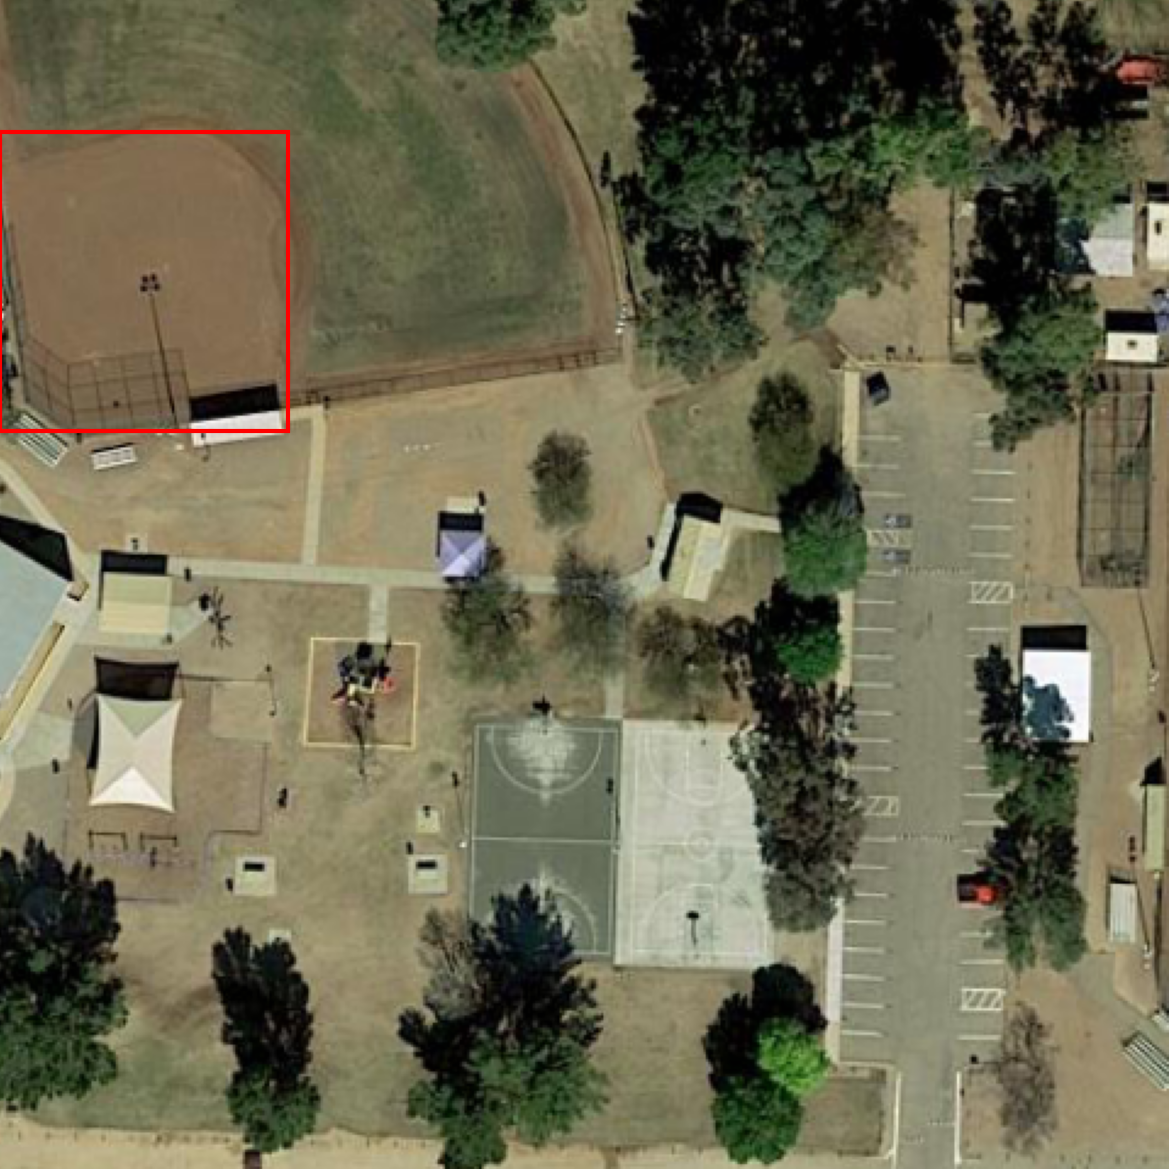
\includegraphics[width=0.65\textwidth]{./images/3llm.png}
\end{minipage}%
\begin{minipage}{0.5\textwidth}
\centering
\hspace{-1cm}
\raisebox{-0.3\height}{%
\footnotesize
\begin{tabular}{@{}p{2cm}p{5cm}@{}}
\toprule
\textbf{Expression Type} & \textbf{Example} \\
\midrule
Original & the orange baseball diamond in the top left \\
\midrule
o3 Enhanced & the orange baseball diamond with the light pole near home plate in the upper left \\
\midrule
Gemma3 Base & the bright orange baseball diamond to the left of another similar baseball diamond in the top left \\
\midrule
Gemma3-Aerial-12B & the orange baseball field with a chainlink fence surrounded by grass to the north and trees to the west \\
\bottomrule
\end{tabular}%
}
\end{minipage}
\caption{Qualitative comparison between o3, vanilla Gemma3 base model, and our fine-tuned Gemma3-Aerial-12B model on aerial imagery. The table shows how each model enhances the original rule-based expression using an identical prompt and decoding setup, demonstrating the progression from basic rule-based descriptions through increasingly capable LLM enhancements.}
\label{fig:distillation_comparison}
\end{figure*}


\subsection{Historic Filter Ablation Study}
\label{subsec:historic_ablation}

In order to understand how much the historic-image filters described in Section~\ref{subsec:historic_filters} contribute to robustness, we repeat the combined training without injecting those filters. Models that only encounter clean, contemporary imagery typically falter when historic photographs suddenly introduce monochrome toning, contrast loss, or sepia casts. We therefore run an ablation that removes the filters from the training mix and compares the resulting model against the full recipe, using the RSRefSeg-b variant because its SAM-ViT-Base backbone trains faster and lets us report results alongside the base model in Table~\ref{tab:combined_training_results}.

Table~\ref{tab:historic_ablation_results} summarises both setups. Each row lists the clean mIoU (Orig.), the historic counterpart (Hist., in \textcolor{blue}{blue}), and the drop relative to the full-training baseline. Removing filters keeps the Orig. values aligned with Table~\ref{tab:combined_training_results} yet costs five to nine points on the historic splits. Excluding Urban1960SatSeg is far more damaging: the model recovers less on the filtered datasets, collapses to roughly 18\% mIoU on Urban1960SatSeg, and loses the only source of direct historic supervision. Synthetic filters therefore help, but real historic imagery remains necessary because Urban1960SatSeg introduces different land-cover labels—such as treating buildings as area classes—and includes considerably more noise than the other datasets.
% Historic filter ablation table
\begin{table*}[t]
\centering
\caption{Historic-filter ablations. Each row lists the clean score followed by the historic-filter variant (blue) with percentage-point deltas relative to Table~\ref{tab:combined_training_results}; the second row also removes Urban1960SatSeg supervision.}
\label{tab:historic_ablation_results}
\renewcommand{\arraystretch}{1.1}
\resizebox{\textwidth}{!}{%
\begin{tabular}{@{}l|cc|cc|cc|c@{}}
\toprule
\multirow{2}{*}{\textbf{Training Setup}} & \multicolumn{2}{c|}{\textbf{RRSIS-D (mIoU)}} & \multicolumn{2}{c|}{\textbf{NWPU-Refer (mIoU)}} & \multicolumn{2}{c|}{\textbf{RefSegRS (mIoU)}} & \multicolumn{1}{c}{\textbf{Urban1960SatSeg (mIoU)}} \\
\cmidrule(lr){2-3} \cmidrule(lr){4-5} \cmidrule(lr){6-7}
 & \textbf{Orig.} & \textbf{Hist.} & \textbf{Orig.} & \textbf{Hist.} & \textbf{Orig.} & \textbf{Hist.} & \textbf{Orig.} \\
\midrule
No Filters & 64.30\% & \textcolor{blue}{55.00\%} (\textcolor{red}{-6.16}) & 39.50\% & \textcolor{blue}{27.50\%} (\textcolor{red}{-5.65}) & 24.80\% & \textcolor{blue}{12.00\%} (\textcolor{red}{-5.54}) & 69.00\% (\textcolor{red}{-1.65}) \\
No Filters + No Urban1960SatSeg & 63.00\% & \textcolor{blue}{56.00\%} (\textcolor{red}{-5.16}) & 38.00\% & \textcolor{blue}{29.00\%} (\textcolor{red}{-4.15}) & 23.50\% & \textcolor{blue}{13.50\%} (\textcolor{red}{-4.04}) & 18.00\% (\textcolor{red}{-52.65}) \\
\bottomrule
\end{tabular}%
}
\renewcommand{\arraystretch}{1}
\end{table*}

Values in parentheses denote percentage-point change relative to the baseline combined model in Table~\ref{tab:combined_training_results}; \textcolor{blue}{blue} marks historic-filtered validation scores.